%%%%%%%%%%%%%%%%%%%%%%%%%%%%%%%%%%%%%%%%%%%%%%%%%%%%%%%%%%%%%%
% --> INTRODUCCIÓN
%%%%%%%%%%%%%%%%%%%%%%%%%%%%%%%%%%%%%%%%%%%%%%%%%%%%%%%%%%%%%%
\section{Introducción}


%%%%%%%%%%%%%%%%%%%%%%%%%%%%%%%%%%%%%%%%%%%%%%%%%%%%%%%%%%%%%%
% --> OBJETIVOS
%%%%%%%%%%%%%%%%%%%%%%%%%%%%%%%%%%%%%%%%%%%%%%%%%%%%%%%%%%%%%%
\subsection{Objetivos}



%%%%%%%%%%%%%%%%%%%%%%%%%%%%%%%%%%%%%%%%%%%%%%%%%%%%%%%%%%%%%%
% --> OBJETIVO GENERAL
%%%%%%%%%%%%%%%%%%%%%%%%%%%%%%%%%%%%%%%%%%%%%%%%%%%%%%%%%%%%%%
\subsubsection{Objetivo General}
\begin{itemize}
\item 
\end{itemize}

%%%%%%%%%%%%%%%%%%%%%%%%%%%%%%%%%%%%%%%%%%%%%%%%%%%%%%%%%%%%%%
% --> OBJETIVOS ESPECÍFICOS
%%%%%%%%%%%%%%%%%%%%%%%%%%%%%%%%%%%%%%%%%%%%%%%%%%%%%%%%%%%%%%
\subsubsection{Objetivos Específicos}
\begin{itemize}
\item 
\item 
\item 
\item
\item 
\end{itemize}

%%%%%%%%%%%%%%%%%%%%%%%%%%%%%%%%%%%%%%%%%%%%%%%%%%%%%%%%%%%%%%
% --> ENUNCIADO
%%%%%%%%%%%%%%%%%%%%%%%%%%%%%%%%%%%%%%%%%%%%%%%%%%%%%%%%%%%%%%
%\newpage

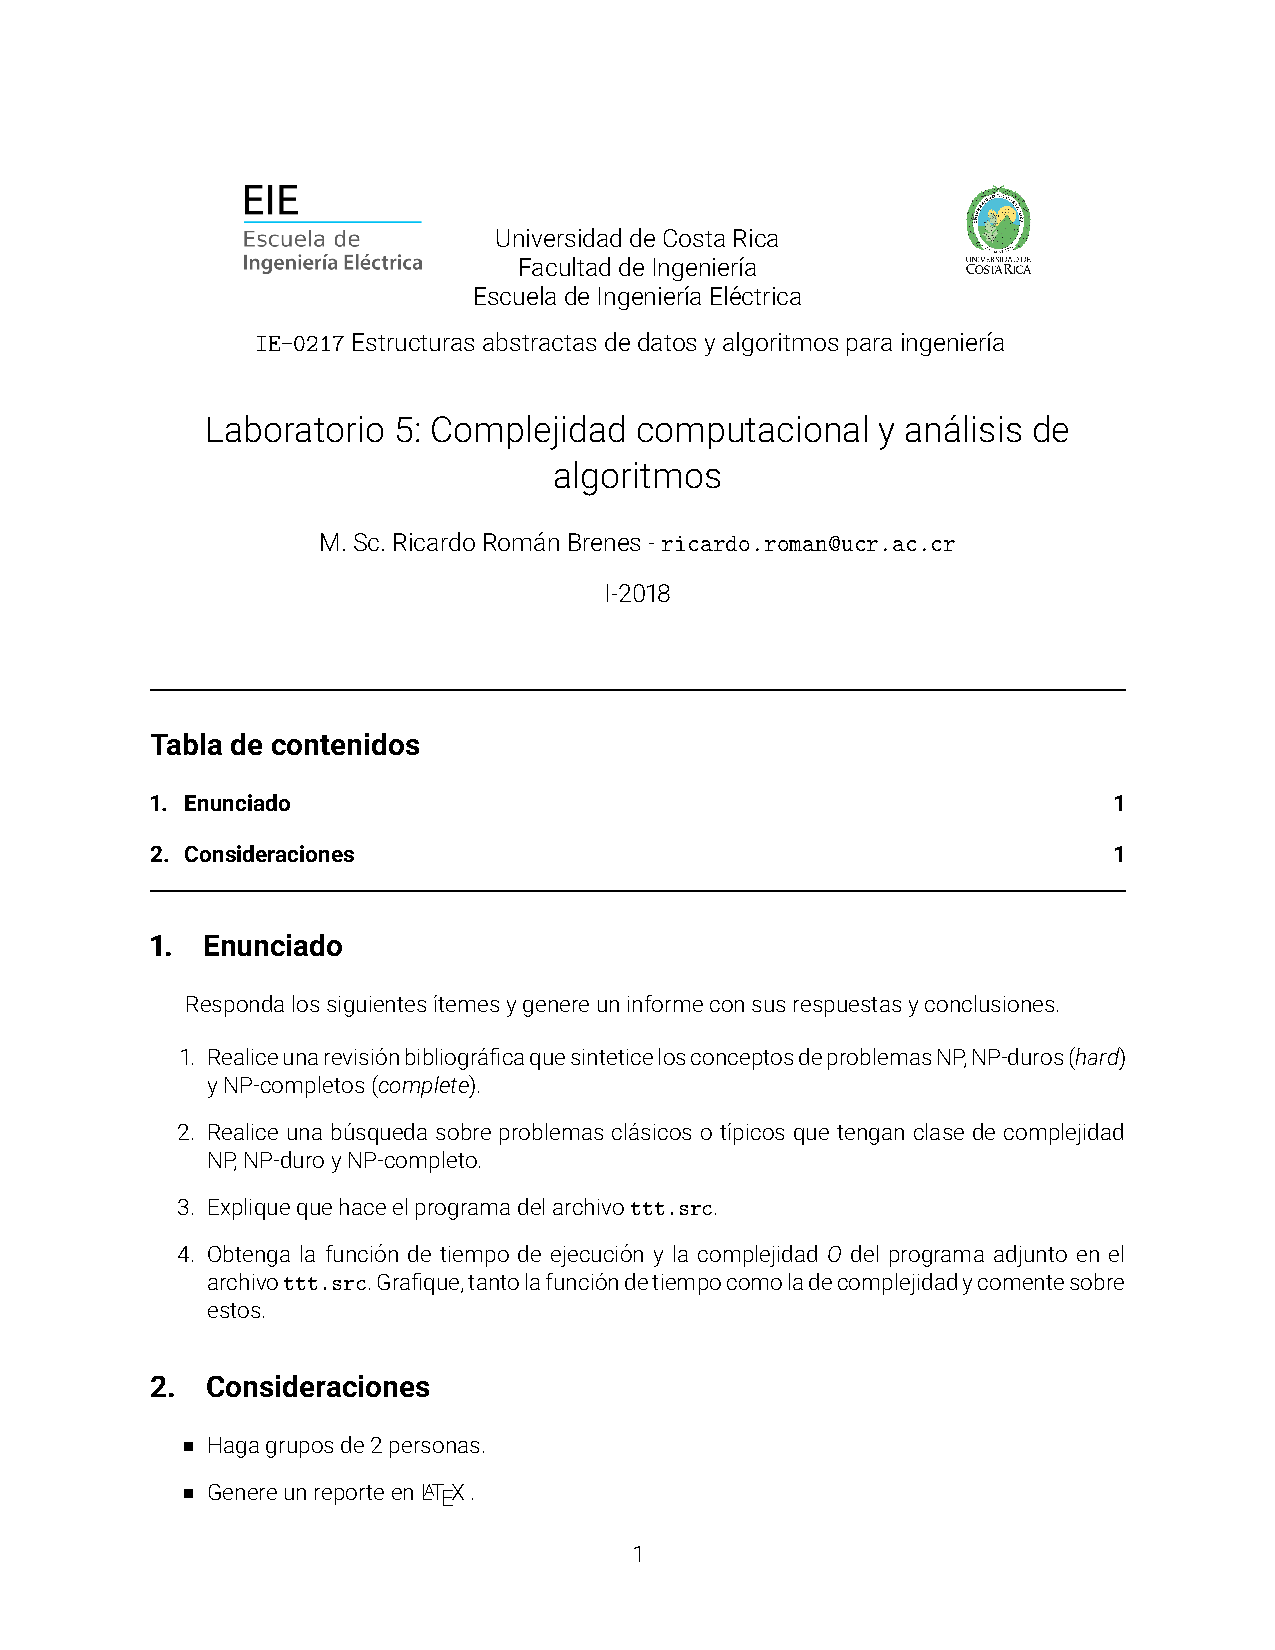
\includepdf[pages=1,pagecommand=\section{Enunciado}, scale=0.8]{enunciados/enun5} 
\includepdf[pages=2,pagecommand={},scale=0.8]{enunciados/enun5}

%%%%%%%%%%%%%%%%%%%%%%%%%%%%%%%%%%%%%%%%%%%%%%%%%%%%%%%%%%%%%%
% --> SOLUCIÓN
%%%%%%%%%%%%%%%%%%%%%%%%%%%%%%%%%%%%%%%%%%%%%%%%%%%%%%%%%%%%%%
\section{Solución}

\subsection{Clases de complejidad computacional}

La complejidad computacional es una rama de la teoría de la computación, y se encarga de medir la dificultad para computar una función en términos de los recursos requeridos, principalmente tiempo y espacio \cite{R3}. Esta teoría plantea una clasificación en \emph{clases}, según la dificultad inherente de los problemas.

Por lo general, un método que se utilice para resolver un problema de decisión se denomina \textit{algoritmo}. Un algoritmo \textbf{de tiempo polinomial} es aquel cuyo tiempo de ejecución crece en función del tamaño de su entrada como una función polinomial \cite{R4}.

%-----------------------------------
\subsubsection{Problemas NP}
%-----------------------------------

En complejidad computacional se pueden presentar problemas no deterministas, estos son problemas que se resuelven en tiempo polinomial no de

%-----------------------------------
\subsubsection{Problemas NP-Hard}
%-----------------------------------
%En la clase NP-Hard son todos aquellos problemas en NP que puede ser polinometicamante reducidos 
%La clase de problemas NP-Hard, por lo general requieren de una solución exponencial e inclusive peor. 


%-----------------------------------
\subsubsection{Problemas NP-Complete}
%-----------------------------------

Existe una clase de problemas NP, de la que se dice que no se conoce su estado. Esto quiere decir que no se ha descubierto ningún algoritmo de tiempo polinomial que resuelva un problema de este tipo, pero tampoco se ha comprobado que no pueda existir alguno \cite{R5}. Se afirma, además, que si \textbf{algún} problema de tipo NP-C se puede resolver en tiempo polinomial, entonces \textbf{cualquier} problema de tipo NP es solucionable con un algoritmo de tiempo polinomial.

\subsection{Análisis del programa en el archivo \texttt{theCode.src}}

\begin{minted}[linenos,autogobble,bgcolor=bg,breaklines,fontsize=\footnotesize ]{c++}
#include <string>
#include <iostream>
using namespace std;

class FileUtil
{
  public:
  	FileUtil(string s, ios_base::openmode p);
  	~FileUtil();
  	string read();
  	string* readLines();
  	int write(string s);
  	int write(string* s, int n);
    void countNumberLines();
    int getNumberLines();
  private:
    //Numero de lineas.
    int numLines;
    //Dirección de lectura.
    string ruta;
    //Modo de lectura.
  	ios_base::openmode modo;
    //Linea leida.
    string line;
    //Puntero con la direccion del arreglo de las lineas leidas.
    string* lines;

};
\end{minted}



%%%%%%%%%%%%%%%%%%%%%%%%%%%%%%%%%%%%%%%%%%%%%%%%%%%%%%%%%%%%%%
% --> RESULTADOS
%%%%%%%%%%%%%%%%%%%%%%%%%%%%%%%%%%%%%%%%%%%%%%%%%%%%%%%%%%%%%%
\section{Resultados}



%%%%%%%%%%%%%%%%%%%%%%%%%%%%%%%%%%%%%%%%%%%%%%%%%%%%%%%%%%%%%%
% --> CONCLUSIONES
%%%%%%%%%%%%%%%%%%%%%%%%%%%%%%%%%%%%%%%%%%%%%%%%%%%%%%%%%%%%%%
\section{Conclusiones}


Como conclusiones se tiene que:

\begin{itemize}
\item 
\item 
\item 
\item 
\end{itemize}


%%%%%%%%%%%%%%%%%%%%%%%%%%%%%%%%%%%%%%%%%%%%%%%%%%%%%%%%%%%%%%
% --> BIBLIOGRAFIA
%%%%%%%%%%%%%%%%%%%%%%%%%%%%%%%%%%%%%%%%%%%%%%%%%%%%%%%%%%%%%%
\begin{thebibliography}{IEEE}
\bibitem{R1} Talens, S. \textbf{\textit{Curso de programación en C++}}. EUI (UPV) Valencia, 17 al 28 de Julio de 1995. 

\bibitem{R2} Raffo, E. \textbf{\textit{Programación genérica en C++, usando Metaprogramación}}. 2007. Sistemas de Informática. 

\bibitem{R3} Immerman, N. \textbf{\textit{Computational complexity classes}}. Encyclopedia of Mathematics, 2011. Visto el 7 de mayo en \url{https://www.encyclopediaofmath.org/index.php/Computational_complexity_classes}

\bibitem{R4} Kaliski B.  \textbf{\textit{Polynomial Time}}. Encyclopedia of Cryptography and Security. Springer, Boston, MA, 2005.

\bibitem{R5} Cormen, T., Leiserson, C., Rivest, R. y Stein, C. \textbf{\textit{Introduction to Algorithms}}. Tercera Ed. Massachusetts Institute of Technology, 2009.

\end{thebibliography}

